\chapter{Проектирование программного обеспечения} \label{ch:ch2}
Современные приложения редко работают в изоляции. Большинство из них общаются друг с другом по сети и координируют свои действия, обмениваясь сообщениями. Таким образом, современная программная система представляет собой набор распределенных приложений, которые работают на разных участках сети и взаимодействуют с помощью различных коммуникационных протоколов. Например, интернет-магазин может состоять из нескольких распределенных компонентов, таких как система управления заказами, каталог, база данных и т. д. Для реализации бизнес-возможностей подобного интернет-магазина необходимо наладить связь между этими компонентам.

С появлением микросервисной и облачно-ориентированной архитектур традиционные приложения, обладающие разными бизнес-возможностями, подверглись разделению на более мелкие, автономные и бизнес-ориентированные сущности, известные как микро- сервисы. И эти микросервисы должны связываться друг с другом по сети, используя методики межпроцессного (межсервисного, межпрограммного) взаимодействия (inter-process communication, IPC). Существует несколько методик для осуществления межсервисного взаимодествия такие как SOAP, REST, RPC и другие. В данной работе выбор пал на методику REST, так как в наше время построение приложений с помощью архитектурного стиля REST вкупе с HTTP и JSON стало фактическим стандартом для создания микросервисов.  На рисунке \ref{fig:sys_architecture} показана архитектура разработанной системы, где Fabric Network и Middleware рассматриваются как отдельные микросервисы, взаимодействующие друг с другом. Все виды взаимодействий инициируются клиентом.
\begin{figure}[ht]
	\centering
	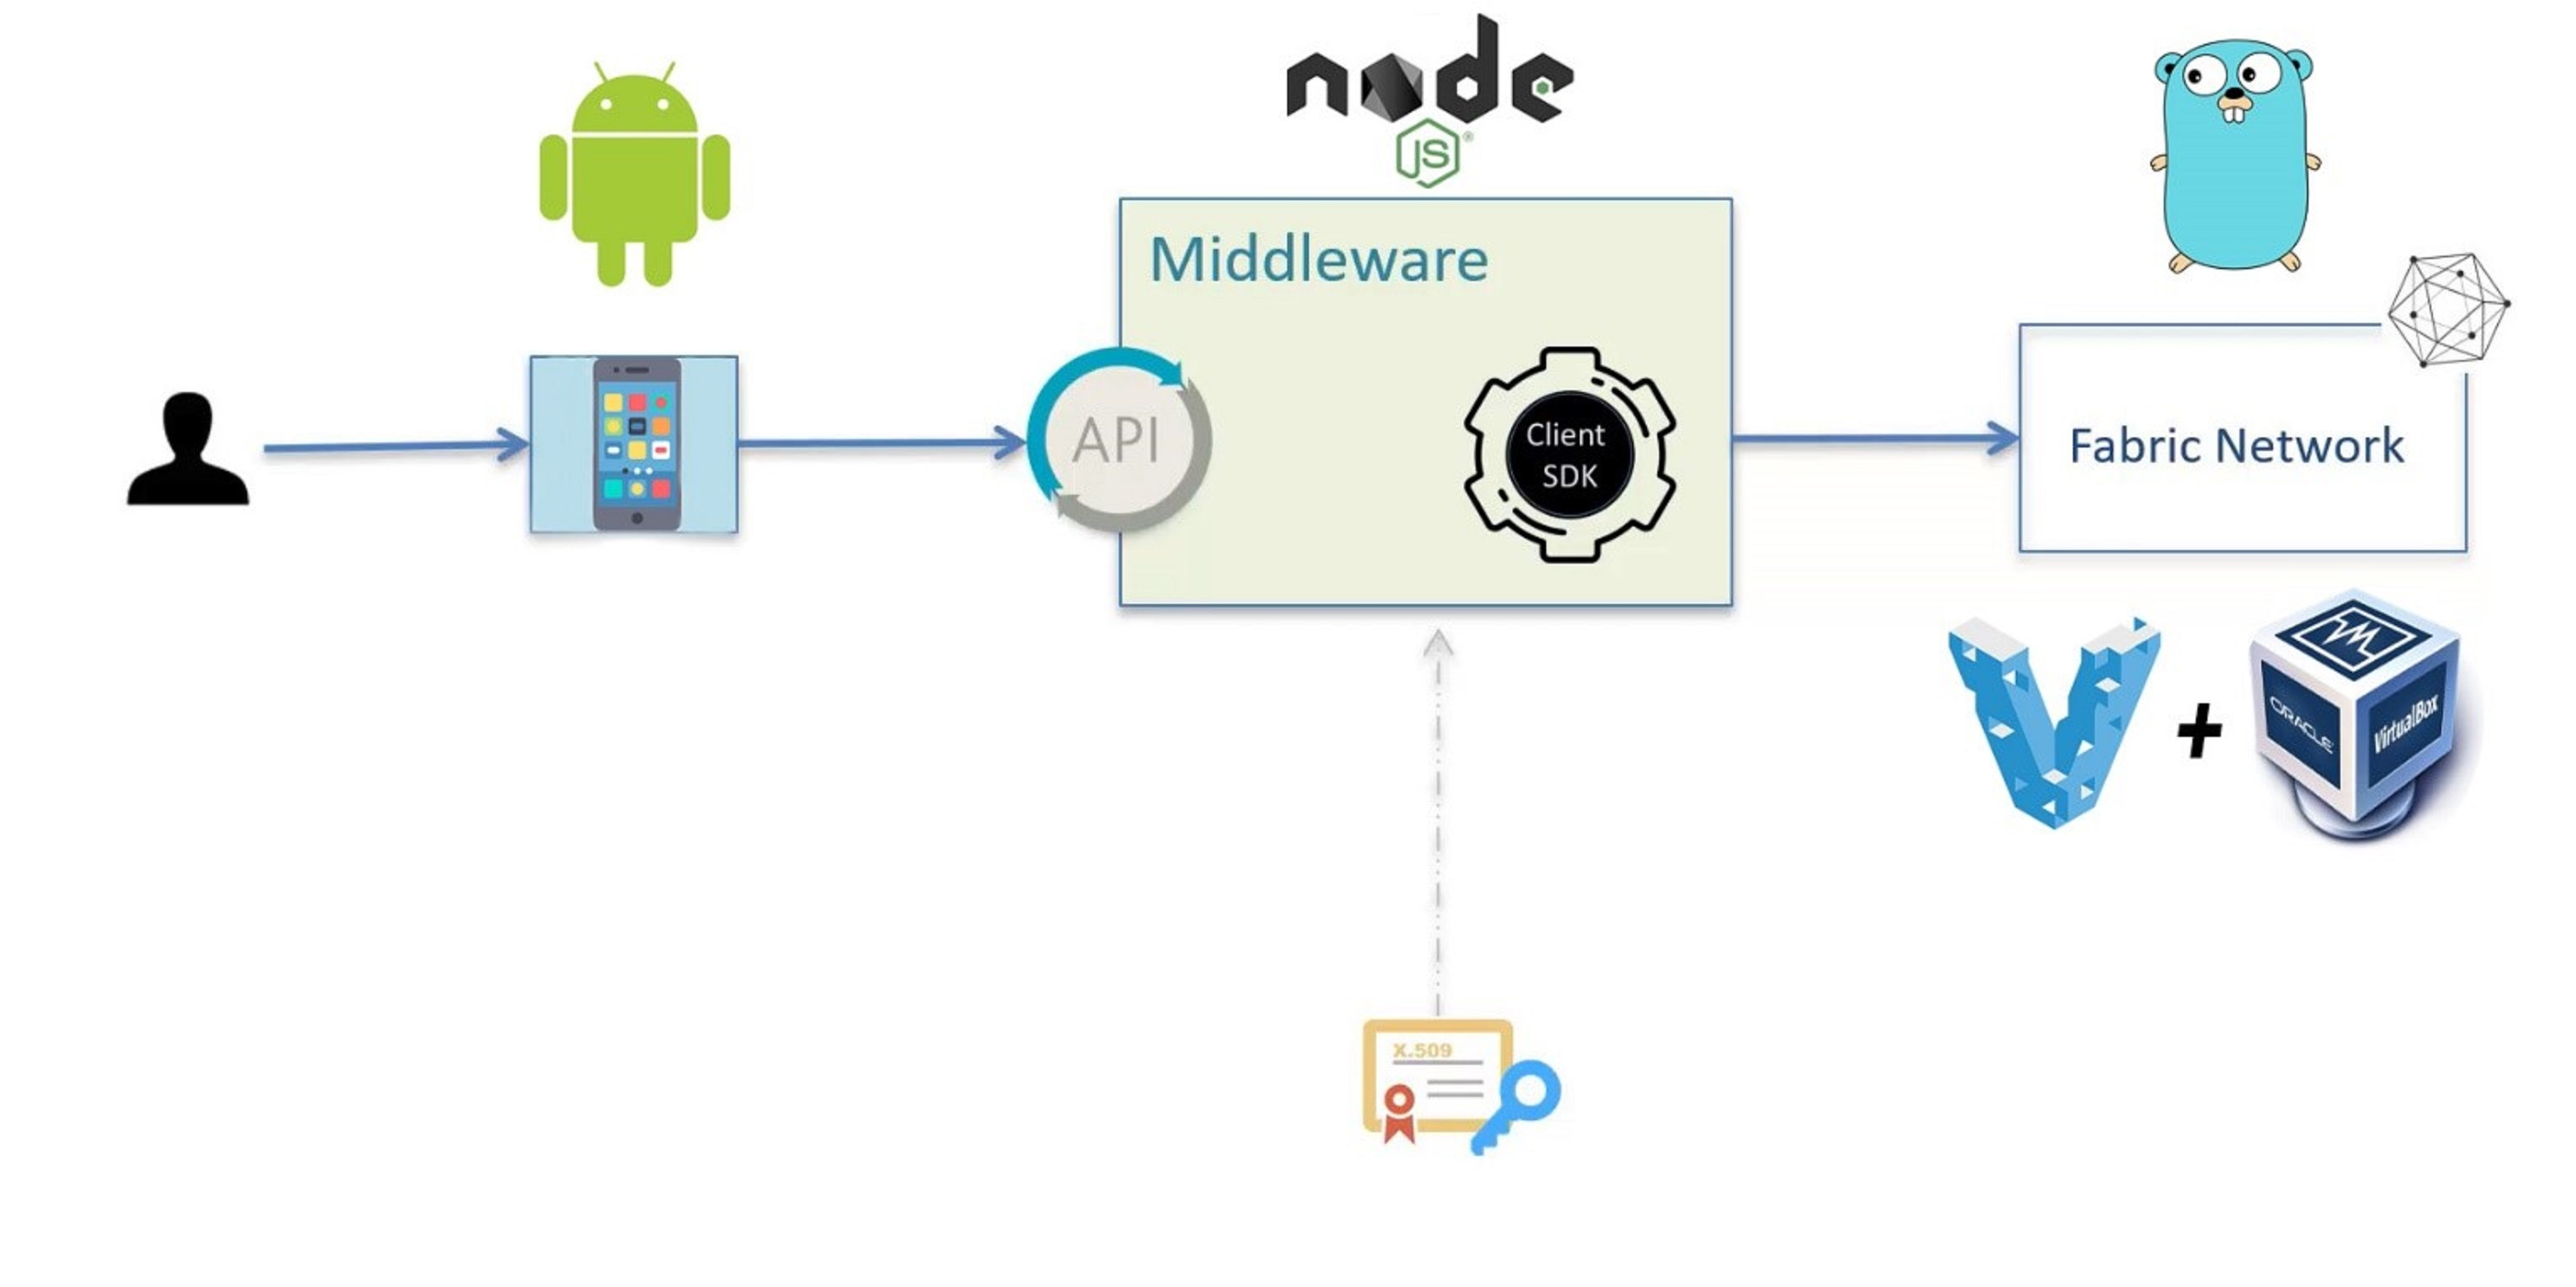
\includegraphics [scale=0.5] {sys_architecture}
	\caption{Архитектура разработанной системы.}
	\label{fig:sys_architecture}
\end{figure}